\documentclass[graybox]{svmult}

\usepackage{mathptmx}       % selects Times Roman as basic font
\usepackage{helvet}         % selects Helvetica as sans-serif font
\usepackage{courier}        % selects Courier as typewriter font
\usepackage{type1cm}        % activate if the above 3 fonts are
                            % not available on your system
\usepackage{makeidx}         % allows index generation
\usepackage{graphicx}        % standard LaTeX graphics tool
                             % when including figure files
\usepackage{multicol}        % used for the two-column index
\usepackage[bottom]{footmisc}% places footnotes at page bottom


% CUSTOM
%\usepackage{amsmath}
%\usepackage{algorithm}
%\usepackage[noend]{algpseudocode}

%\usepackage{mathpartir}
\usepackage{booktabs}
%\usepackage{graphicx}
%\usepackage{graphics}
%\usepackage{geometry}

\usepackage{listings}
\usepackage{xcolor}
\usepackage{anyfontsize}

\definecolor{codegreen}{rgb}{0,0.6,0}
\definecolor{codegray}{rgb}{0.5,0.5,0.5}
\definecolor{codepurple}{rgb}{0.58,0,0.82}
\definecolor{backcolour}{rgb}{0.95,0.95,0.92}
\lstdefinestyle{mystyle}{
    backgroundcolor=\color{backcolour},
    commentstyle=\color{codegreen},
    keywordstyle=\color{magenta},
    numberstyle=\color{codegray},
    stringstyle=\color{codepurple},
    basicstyle=\ttfamily\footnotesize,
    breakatwhitespace=false,
    breaklines=true,
    captionpos=b,
    keepspaces=true,
    numbers=left,
    numbersep=5pt,
    showspaces=false,
    showstringspaces=false,
    showtabs=false,
    tabsize=2
}
\lstset{style=mystyle}

% see the list of further useful packages % in the Reference Guide

\makeindex             % used for the subject index
                       % please use the style svind.ist with
                       % your makeindex program

%%%%%%%%%%%%%%%%%%%%%%%%%%%%%%%%%%%%%%%%%%%%%%%%%%%%%%%%%%%%%%%%%%%%%%%%%%%%%%%%%%%%%%%%%

\begin{document}

\title*{OAGRE: Outlier Attenuated Gradient Boosted Regression}
\titlerunning{OAGRE: Outlier Attenuated Gradient Boosted Regression}
\author{John Hawkins}
\authorrunning{John Hawkins}
\institute{John Hawkins \at Transitional AI Research Group \& Getting-Data-Science-Done.com, (Sydney, Australia),
 \email{john@getting-data-science-done.com}}
\maketitle

\abstract*{Gradient boosting is a general machine learning technique for iteratively building 
a model by fitting the residuals of an existing model.
In spite of its genrality as a technique, there are several reasons why gradient
boosting may fail to adequately model a given dataset. One of these reasons is the presence of 
excessive noise in the training data. In this paper we propose a technique that will
mitigate the impact of noise under some conditions of heteroscedasticity.
We break the assumption of independently distributed noise and derive a simple variation of
the gradient boosting algorithm we name Outlier Attenuated Gradient Boosting Regression (OAGRE).
We conduct experiments by generating large volumes of synthetic datasets with varying
degrees of heteroscedasticity and benchmark our approach against multiple standard gradient
boosting algorithms as well as simpler tree models. 
Our approach provides value in approx 30\% of these synthetic datasets with an average improvement
of between 7\% and 12\% lower root mean squared error. Based on these results we recommend the
inclusion of the OAGRE method when testing algorithms on data with suspected heteroscedasticity issues.}
  
\abstract{Gradient boosting is a general machine learning technique for iteratively building
a model by fitting the residuals of an existing model.
In spite of its genrality as a technique, there are several reasons why gradient
boosting may fail to adequately model a given dataset. One of these reasons is the presence of
excessive noise in the training data. In this paper we propose a technique that will
mitigate the impact of noise under some conditions of heteroscedasticity.
We break the assumption of independently distributed noise and derive a simple variation of
the gradient boosting algorithm we name Outlier Attenuated Gradient Boosting Regression (OAGRE).
We conduct experiments by generating large volumes of synthetic datasets with varying
degrees of heteroscedasticity and benchmark our approach against multiple standard gradient
boosting algorithms as well as simpler tree models.
Our approach provides value in approx 30\% of these synthetic datasets with an average improvement
of between 7\% and 12\% lower root mean squared error. Based on these results we recommend the
inclusion of the OAGRE method when testing algorithms on data with suspected heteroscedasticity issues.}


\section{Introduction}

Gradient Boosting has proven itself to be one of the most significant advances in
the field of machine learning in recent history. Its utility in providing accurate predictions
for supervised learning is so strong that it has come dominate the field of competitive machine 
learning on tabular datasets (as explified by the competitions run by Kaggle \cite{kaggle}).
In spite of its success, there remain a range of specific circumstances which limit the ability of
gradient boosting (and other algorithms) to provide adequate reaults. One of these
circumstances is the presence of complex noise in the data.
Early boosting algorithms, like AdaBoost, were known
to suffer in the presence of noise \cite{Freund2001,Schapire2003}. Modern gradient boosting
algorithms are less susceptible to these issues and tend to perform well with small amounts of
heteroskedastic noise \cite{brophy2022}. However, there is always potential for learning issues
to emerge if some of the residuals become dominated by the presence of noise.

Gradient boosting algorithms are predeominantly tree based and there are multiple variations 
offering improvements in performance and comptational efficiency, typically through the way variables
are selected and the base learners are combined \cite{Ke2017}.
However, in all cases the theoretical underpinnings of the gradient boosting algorithm
remain unchanged. The algorithm consists of learning an ensemble of base learners
as an additive combination. In each iteration the new model is trained to predict the
residuals of the preceding ensemble \cite{Friedman2000,Friedman2001,Friedman2002}. 

In this paper we develop a variation of the gradient boosting algorithm by making
several non-standard assumptions about the noise present in the data.
This involves breaking the assumption that the noise is identically distributed across the
problem space. In particular we assume that the distribution of the noise varies in a way that
can be at least partially predicted by the known regressors for the machine learning problem.

Noisey data with hetereoscedasticity has been shown to be deleterious to regression trees (the most
common base learner for gradient boosting models) \cite{ruth2016effect}. In addition, there are
many application domains in which the noise is known to be hetereoscedastic, and the focus of
research is to develop custom algorithms that explicitly model the noise variance \cite{Zhenxing2020,Zhang2023},
or build custom ensembles where subcomponents are used to accomodate the hetereoscedasticity \cite{Zeng2022}. 
Common general machine learning approaches include the development
of noise filtering or re-labelling techniques, under the assumption that the noisy data is an
outlier to be detected \cite{Ustinovskiy2016}. Other research has focused on modification of the base 
learners in ensemble methods (including gradient boosting ensembles) to make them more robust to 
hetereoscedasticity \cite{Henrey2016}, or to attempt to explicitly model the heteroscedastic noise
distribution \cite{Natarajan2009,Thomas2018} and incorporate the noise distribution into the loss function to 
weight samples accordingly \cite{Lee2017}. 
An alternative approach has been to augment the design of the gradient boosting method 
by quantifying the uncertainty in the predictions generated by the heteroscedasticity \cite{brophy2022},
or to model the output distribution directly using quantile or expectile regression \cite{Yang2014}.
In situations in which
there is known noiseless data, or it can be simulated, then there are techniques that allow models to
be trained such that they are influenced less by the noise distribution \cite{Wu2021}. However, as our 
ability to fit models depends heavily on the amount of data and the nature of the noise, which is usually
unknown, heteroscedasticity remains an open problem for machine learning research.

In this work we explore the extent to which assuming hetereoscedastic noise in a dataset can be used
to derive a fundamental variation of the gradient boosting algorithm. 
The core idea is that if the noise distribution is variable then high noise regions of the problem space should be fit with simpler
models than the low noise regions. Such that the model does not waste computational resources fitting
noisy data points. The gradient boosting is selectively applied by predicting whether a given sample
belongs to a region that surpasses the noise threshold for each level of the boosted model.

To do so we assume that there will be some correlation between the magnitude of the error made
by the model and the presence of higher variance noise. This assumption requires only that our feature
vector and model be rich enough that we expect the model to be able to learn the
relationship between dependent and independent variables well enough that noisier samples stand out.
In the absence of noise we expect error to be low, when noise is present we expect it to be high.
Because the first assumption gives us non-uniform noise, we therefore expect the presence
of a noise gradient that is correlated with the error.

Combining these two assumptions with the learning strategy of gradient boosting for regression, leads us to an
alternative formulation of the gradient boosting algorith. The core idea being that each iteration of boosting should
seek to learn only from residuals that come from regions in the parameter space that contain less noise. In other
words we predict which samples are noisier outliers and exclude them from the training of subsequent models in the
ensembnle. We call this algorithm Outlier Attenuated Gradient Boosting Regression (OAGRE)

\section{Method}

We start the derivation of the method by assuming that the noise is not randomly distributed with respect to the
features or predictors, but instead is predictably heteroscedastic.
This assumption is contrary to the standard expression for the learning problem,
an example of which is shown in Equation \ref{eq:noise} taken from Friedman 2000 \cite{Friedman2000}.

\begin{equation}
y_i = F^*(X_i) + \epsilon_i
\label{eq:noise}
\end{equation}

This expression defines the target variable of instance $i$,$y_i$ as a function of the features vector $X$
plus some Gaussian noise $\epsilon_i$. It is generally assumed that the noise term is independent of the 
feature vector $X$. It may correspond to inherent noise, or be due to unobserved causal factores that are
not present in the features, and hence limit our ability to perfectly represent the target using the given
features.
 
We modify this assumption in the following way: the noise term $\epsilon_i$ is partially dependent upon the
feature vector $X_i$, but only in its variance. In real world processes there are multiple reasons
why noise might be correlated with predictors. Noise can come from sampling problems,
which are not uniformly distributed. Noise might be due to limitations of the devices
or methodology used to collect data, which again tend not to be uniformly distributed.
Most noise is due to some physical process, which itself is regulated by variables,
if any of the variables that regulate the noise are present as features then we should 
expect the statistical structure of the noise to vary over the features space.

This means that we should expect the learning problem in many real world problems to be
%
\begin{equation}
y_i = F^*(X_i) + \epsilon(N(X_i))
\label{eq:noisytarget}
\end{equation}
%
in which $\epsilon(N(X_i))$ refers to a sample drawn from a noise distribution $N$ that is
dependent on the independent variables of the sample $X_i$.

When we are training a model to predict $y_i$, then we typically depict the fit of the model
using a similar equation.

\begin{equation}
\hat{y}_i = \hat{F}(X_i)
\label{eq:fit}
\end{equation}

Such that the function $\hat{F}$ has been fit such that given a feature vector $X_i$ it provides an estimate of $y_i$.
The error of such a model can be calculated for each record as the difference between the actual and predicted value:

\begin{equation}
err_i = y_i - \hat{y}_i
\label{eq:error}
\end{equation}

Note that error is typically calculated using some loss function $L(y,\hat{y})$, however we will ignore that complication for the moment.
We can substitute Equations \ref{eq:noisytarget} and \ref{eq:fit} into Equation \ref{eq:error} and with some rearrangement end up
with the following expression for the error:

\begin{equation}
err_i = ( F^*(X_i) - \hat{F}(X_i) )  + \epsilon(N(X_i))
\label{eq:noisyerror}
\end{equation}

In other words the expected error in our model is the difference between the true underlying function and the estimated one,
plus the expected noise in that region of the problem space.

For many algorithms the change we have made to the distribution of noise is not something that can easily be exploited.
However, the gradient boosting algorithm has the potential to exploit this new feature of the problem. Usually noise undermines
a gradient boosting step because it is attempting to use the residual of the existing model to build a new iteration that
improves the previous model. One might imagine that at some point the residuals come to be dominated by the noise term, and hence a
gradient boosted algorithm cannot see the signal for the noise.

If however, the noise is not identically distributed across the feature space then we could potentially direct each round of
gradient boosting to ignore noisy examples, and focus on learning from a subset of the data. This is similar to what Freund
did in the development of BrownBoost \cite{Freund2001}, a generalisation of AdaBoost, although in his treatment it involved
setting an expected minimum error rate and then smoothly downweighting samples that exceeded this threshold.

In order to modify the learning algorthm to ignore samples suspected of being dominated by noise we need to provide some
kind of selection criteria for deciding at the start of each iteration which samples to exclude.
We introduce an additional threshold meta-parameter which determines when an example should be ignored. This parameter
determines the threshold in the standard deviation of the resisual errors beyond which a sample is considered an outlier.
In addition we allow this parameter to be adjusted downward with each iteration of learning, so that the model 
increases the volume of samples that are treated as outliers as the boosting ensemble grows.

In order to apply the model to new data we cannot simple make predictions using all stages of the gradient boosting because
deeper level trees have been trained only samples from a subset of the feature space. In other words, our gradient boosted model
covers the problem space at different levels of granularity, depending on our expectations of the noise distribution.
We only apply each subsequent gradient boosting model in a way that it is attenuated according to our estimate of
whether or not it is appropriate. We do this by fitting a classification model at each stage of gradient boosting which predicts
whether or not a given example belongs to the signal set (of relatively low noise examples). We use the classifier to
build a model to estimate the probability that sample $i$ is considered to be low noise at depth $j$ in our gradient 
boosted model: $p_j(low noise | X_i )$.

The final prediction can be calculated according to the following formula:
%
\begin{equation}
\hat{y}_i = \hat{B}(X_i) - \sum_{j=1}^M p_j(low noise | X_i) * \hat{R}_j(X_i)
\label{eq:pred}
\end{equation}
%
where $M$ is the parameter defining the number of models in the ensemble, $\hat{B}$ is the base regression model fitted to the
entire dataset, and $\hat{R}_j$ is the estimate of the residuals at depth $j$ of the boosting.
Our prediction $\hat{y}_i$ is a combination of the base model with the negative sum of all residual estimates over the $M$ 
levels of boosting each of which is attenuated by the estimate of the probability that the sample is a low noise example at that 
depth of the boosted model.

\subsection{Implementation}
 
\begin{lstlisting}[language=Python,label={code:skl}, caption=Usage of OAGRE with scikit-learn models ]
from sklearn.tree import DecisionTreeClassifier
from sklearn.tree import DecisionTreeRegressor
from oagre import OAGRE

oagre = OAGRE(
    classifier=DecisionTreeClassifier(max_depth=5),
    regressor=DecisionTreeRegressor(max_depth=5)
)

oagre.fit(X_train, y_train)
...
\end{lstlisting}

We have implemented the OAGRE method as a meta-learning algorithm compatible with scikit-learn \cite{pedregosa2011scikit},
and made it available as an open source python library in the GitHub repository (https://github.com/john-hawkins/oagre).
The implementation requires that the user provide two base models, a classifier and a regressor, which it then uses to
building the gradient boosted ensemble. We show an example of how to instatiate and train an OAGRE regressor in
Listing \ref{code:skl}, where we use the sklearn DecisionTree models for the base classifier and regressor.

Our implementation allows an OAGRE ensemble model to be included inside the machine learning framework
scikit-learn pipelines \cite{pedregosa2011scikit}. The advantage of the pipeline approach is that an OAGRE model 
can be built into a single serialised model for deployment, including data preprocessing stages.
The OAGRE library can be installed as a package from the PyPi repository (https://pypi.org/project/oagre)
or installed directly from the source code (https://github.com/john-hawkins/oagre).
 
\subsection{Evaluation}

To evaluate the effectiveness of our approach we conduct an experiment in which large volumes of synthetic data
sets are created with varying parameterisation of the hetereoscedasticity in the error term. The parameters of
the simulation are shown in Table \ref{tab:sim}. We generate $100$ random datasets for each combination of 
parameters, such that the independent variables are drawn from a range of different numercial distributions
and the target variable is created through a randomly generated formula combining linear and non-linear 
combination of a random subset of independent variables. We generate a second random function that is fed
through a logistic function to create a probability distribution. The outputs of this probability distribution
is used to determine which datapoints will be subject to excessive noise, thus ensuring that the data is
not onluy hetereoscedastic, but that this property is partially dependent on the independent variables.

Once the data is generated we take a random split of 90\% for training and 10\% for testing. 
We train six models for evaluation and comparision. The first two are standard implementations of
the Gradient Boosted Tree algorithm, the GBM model built into the scikit-learn package, and
the LightGBM model \cite{Ke2017}. For each of these models we train them use default parameters,
in order to reduce the computational complexity of performing hyperparameter tuning over large volumes of synthetic
data. The second two models are OAGRE ensembles using different base learners. The first is trained with an 
ExtraTrees model (a Random Forest Implementation) and the second with a DecisionTree model, both of these are
taken from the standard scikit learn implementation. Finally, we included the base regression models used
by the two OAGRE models for comparison, to ensure that the OAGRE algorithm was adding value to these models.
The standard GBM models were initialised with default paramaters, the other models were initialised shown in 
Table \ref{tab:models}. These initialistions are based on our experience with applying the OAGRE technique.
Note, that when using the ExtraTrees model as a base learner, ther number of estimators is a combination of
the estimators used by ExtraTrees and the estimators used in the boosting layers of OAGRE.

\begin{table}
\caption{Simulation Parameters}
\label{tab:sim}
\resizebox{\columnwidth}{!}{%
\begin{tabular}{|l|l|r|}
\toprule
Parameter            &Description                                   &Values     \\
\midrule
Dataset Size         &Number of records in the dataset              &2000, 5000, 10000   \\
Variables            &Number of independent variables               &15, 20, 25, 30      \\
Outlier Proportion   &Proportion of records with larger noise       &0.4, 0.5, 0.6, 0.7  \\
Std Multiplier       &The factor applied to noise std of outliers   &random int(3,8)     \\
\bottomrule
\end{tabular}
}
\end{table}

The complete code for the simulation and evaluation is provided in our GitHub repository. We note that as the
generation of random formulas sometimes produced null values, there is significant checks in place to regenerate
data when problematic scenarios occur. In total this process produced $2,185$ datasets that the models were
trained and evaluated on.

\begin{table}
\caption{Models and Initialisation Parameters}
\label{tab:models}
\resizebox{\columnwidth}{!}{%
\begin{tabular}{|l|l|r|r|}
\toprule
Model             &Description               &Estimators  &Max Depth    \\
\midrule
GBM               &SKLearn GB Regressor      &100       &3              \\
LGBM              &LightGBM                  &100       &Unbounded      \\
OARGE-DT          &OAGRE with DecisionTrees  &20        &5              \\
OAGRE-XT          &OAGRE with ExtraTrees     &200       &5              \\
XTR               &ExtraTrees Regression     &10        &5              \\
DTR               &DecisionTree Regression   &1         &5              \\
\bottomrule
\end{tabular}
}
\end{table}


\section{Results}

In Table \ref{tab:results} show the proportion of datasets for which each model provided the best result (measured
in terms of lowest Root Mean Squared Error). In addition, we show the average percentage improvement of each model against
the next best model for the task. As we see, the overall winner is the standard Gradient Boosting Machine implementation
from the scikit-learn library. The two OAGRE implementations provide a superior model in approx $30\%$ of datasets, with
the version using ExtraTrees models as the base learner showing stronger performance, both in terms of the proportion
of times it is superior, and the expected percentage of improvement. The two base models alone are only superior in a
small percentage of instances, with a more marginal improvement. 

\begin{table}
\caption{Overall Results}
\label{tab:results}
\resizebox{\columnwidth}{!}{%
\begin{tabular}{|l|l|r|r|}
\toprule
Model             &Total Wins   &Percentage of Wins    &Average Improvement    \\
\midrule
GBM               &890       &40.7\%                   &30.8\%              \\
LGBM              &274       &12.5\%                   &25.4\%              \\
OARGE-DT          &279       &12.7\%                   &11.6\%              \\
OAGRE-XT          &430       &19.7\%                   &7.3\%               \\
XTR               &131       & 6.0\%                   &2.5\%               \\
DTR               &180       & 8.2\%                   &2.4\%               \\
\bottomrule 
\end{tabular}
}
\end{table}

\begin{figure*}
\centering
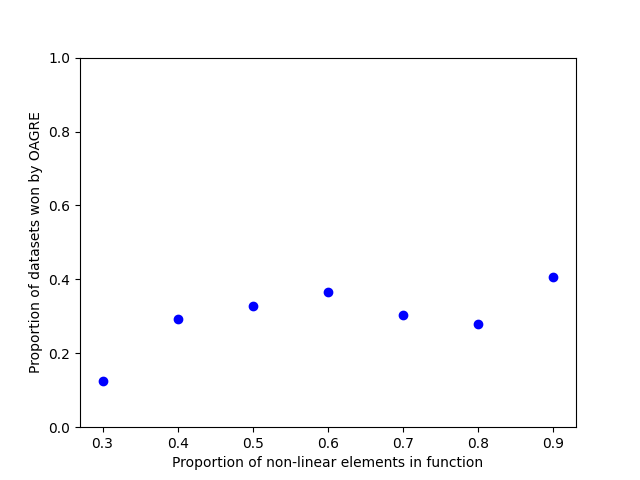
\includegraphics[scale=0.7]{images/wins_vs_nonlinear_prop.png}
\caption{OAGRE Wins against Non-linear Elements in Target Function}
\label{fig:nonlinear}
\end{figure*}

We took the parameters that generated these synthetic datasets and analysed multiple factors that might contribute
to the circumstances in which the OAGRE approach added value. This included the outlier proportion and standard deviation
multiplier factor used to generate the data, as well as the proportion of non-linear elements used in the random formula that
generated the target variable. We observed that the proportion of datasets upon which OAGRE provided superior performance
appeared to be increasing with the proportion of the generating function that was non-linear, as shown in Figure \ref{fig:nonlinear}.

\section{Conclusion}

By questioning a standard assumption in the defintion of regression problems, pertaining to the nature of the noise 
present in a data set, we have been able to derive a variation of the gradient boosting algorithm. Our variation 
compensates for the presences of heteroscedasticity by explcitly modelling the probability that a data point comes
from a high noise region of the data space, and then excluding it from the residual estimates in the boosting process.
We incorporate the probability of a data point being a noisy outlier at prediction time to attentuate the impact of 
residual estimates in the boosting process. 
The resulting meta-learning approach to building an ensemble we call Outlier Attenuated Gradient
Boosting Regression and we release it as a scikit-learn compatible open source library. 

We conducted a simulation based experiment in which we generated large volumes of datasets with hetereoscedastic noise
imposed through parameteristation. These experiments indicate that our approach will provide superior
performance to standard gradient boosting implementation in approx 30\% of cases, with an average reduction in root mean
squared error of between 7\% and 12\% (compared to the next best model). 
We note that this work was done using default parameters to limit the complexity of the search space, hence the impact of 
significant parameter tuning is unknown, but would likely to shift some of these results. Nevertheless, we observe that the 
proportion of instances in which the OAGRE approach proved superior was approximately equal to its proportion in the set of 
methods tested. Hence, we conclude that the technique will likely provide value for some regression problems with heteroscedastic
noise. For this reason we recommend that practitioners facing a regression problem with noiesy heteroscedastic data include the
OAGRE algorithm within a set of empirically evaluated methods. 

Future research could be conducted to determine the exact properties of a dataset that make it amenable to our technique. 
However, preliminary analysis suggests that the more non-linear the function that is being estimated, the greater the likelihood that
OAGRE will provide predictive value.

\bibliographystyle{ieeetr}
\bibliography{refs}

\end{document}
